\genHeader

The toughest part of learning a new language  is often building up a sufficient vocabulary.
This is usually accomplished by repeating a long list of words again and again until they stick.
A \emph{Leitner's learning box}\footnote{http://en.wikipedia.org/wiki/Leitner\_system} is a simple but ingenious little contraption to support this tedious process of memorization.

As depicted in Fig.~\ref{fig:membox_illustration}, it consists of a series of compartments or partitions usually of increasing size.
The content to be memorized is written on a series of cards  which are initially placed in the first partition.
All cards in the first  partition should be repeated everyday and cards that have been successfully memorized are placed in the next partition.
Cards in all other partitions are only repeated when the corresponding partition is full and cards that are  answered correctly are moved one partition forward in the box.
Challenging  cards that have been forgotten are treated as brand new cards and are always  placed right back into the first partition regardless of how far in the box they  had progressed.

These ``rules'' are depicted by the green and red arrows in  Fig.~\ref{fig:membox_illustration}.
The basic idea is to repeat difficult cards as often as necessary and not to waste time on easy cards which
are only repeated now and then to keep them in memory.
The increasing size of the partitions represents how words are easily placed in our limited short term memory and slowly move in our theoretically unlimited long term memory if practised often enough.

%\usepackage{graphics} is needed for \includegraphics
 \begin{figure}[htp]
 \begin{center}
   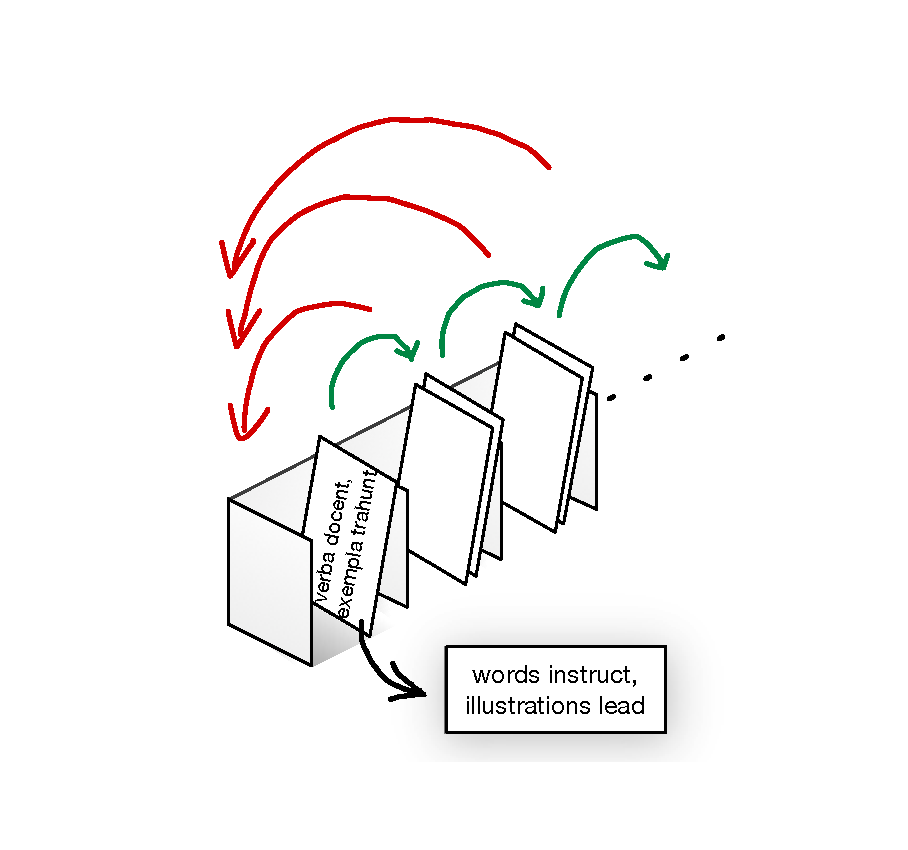
\includegraphics[width=0.5\textwidth]{../membox_illustration}
   \caption[]{Possible \emph{Concrete Syntax} of a Leitner's Learning Box.}
   \label{fig:membox_illustration}
 \end{center}
 \end{figure}
 \FloatBarrier

A learning box is an interesting system, because it consists clearly of a static structure (the box, partitions with varying sizes, and cards with two sides and corresponding content) and a set of rules that describe the dynamic aspects
(behaviour) of the system.
In this Part I handbook, we shall build a complete learning box from scratch in a model-driven fashion and use it to introduce fundamental concepts in metamodelling and \emph{Model-Driven Software Development} (MDSD) in general.
